\chapter{\epigeneticstitle}
\label{chap:epigenomics}
\glsresetall
\clearpage

\section{Introduction}

In the previous chapter, we examined the RCMB56-ht patient tumor and showed that high-copy ecDNA defined a subpopulation of tumor cells expressing a distinct transcriptional program. In this chapter, we examine transcriptional dysregulation which occurs on and around the ecDNA amplified sequences of the RCMB56-pdx and D458 \gls{MB} models as well as several patient tumors. Gene transcription is frequently regulated by distal regulatory elements (enhancers) located up to 1Mbp away \cite{pennacchio_2013}. In some medulloblastomas \cite{northcott_2014} and other cancers \cite{neoloopfinder}, a somatic structural rearrangement (structural variant, SV) may juxtapose an oncogene and an ectopic enhancer to activate oncogenic transcription. Comparing the enhancer landscapes of the Group 3 MB cell lines D458 (\textit{MYC} ecDNA) and D283 (\textit{MYC} \acrshort{HSR}), we observe functional differences in the enhancer loci driving oncogene expression, indicating that the enhancer landscape of the structural variant contributes to oncogenic transcriptional dysregulation. These results add to accumulating evidence suggesting co-amplified enhancers as potential therapeutic vulnerabilities in ecDNA-amplified cancers \cite{hung_2021}.

\section{Results}

\subsection{ecDNA places oncogenes in new gene regulatory contexts.}
It has been shown that some MB tumors are driven by ``enhancer hijacking'' events, whereby somatic SVs cause an enhancer to be rewired to amplify transcription of \textit{GFI1} family or \textit{PRDM6} genes \cite{northcott_2012,Northcott_2017}. Given the extensive genomic rearrangement associated with some MB ecDNA, we investigated whether new DNA interactions between co-amplified non-coding regulatory enhancers and oncogenes emerge on circular ecDNA. To test this hypothesis, we profiled the accessible chromatin of 25 MB tumors (11 ecDNA+, 14 ecDNA-) using ATAC-seq \cite{atac-seq}, as well as chromatin interactions of 17 MB tumors (8 ecDNA+, 9 ecDNA-) using chromatin conformation capture (Hi-C) \cite{rao_2014}. Consistent with previous reports \cite{Wu_2019,kumar_2020}, bulk ATAC-seq read density was markedly enriched across entire ecDNA regions, even for ecDNA with only low-level amplification as estimated by bulk WGS. Hi-C sequencing reads exhibited a similar pattern of enrichment at ecDNA regions (Fig. \ref{fig:mb106-mb248-myc-hic}). 

\begin{figure}[!h]
    \centering
    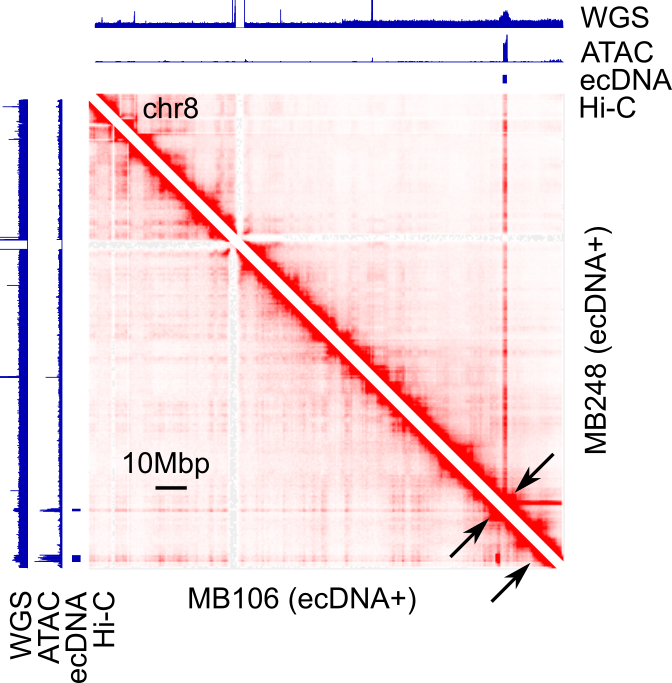
\includegraphics{MB106-MB248-chr8}
    \label{fig:MB106-MB248-hic}
    \caption[Chromatin interaction maps of chr8 in patient tumors with \textit{MYC} ecDNA.]{\textbf{Chromatin interaction maps of chr8 in patient tumors with \textit{MYC} ecDNA.} Chromosome-wide view of intrachromosomal interactions mapping to chr8 of the reference human genome. \Gls{wgs}, ATAC-seq and Hi-C sequencing depth are shown for two Group 3 MB samples harboring circular amplification of \textit{MYC}. Extrachromosomally amplified loci are indicated by arrows. These tumors are described further in \cite{archer_2017}.
    }
    \label{fig:mb106-mb248-myc-hic}
\end{figure}

\par In half of the analyzed ecDNA+ tumors (D458, MB106, MB268, and RCMB56), we observed clear evidence of aberrant chromatin interactions on ecDNA which spanned DNA breakpoints to link accessible loci and co-amplified genes from distal genomic regions. In the \textit{MYC}-amplified Group 3 MB primary tumor MB106, DNA interactions occurred between the \textit{MYC} locus and two co-amplified accessible regions located 13Mbp away on the reference genome, but 75kbp and 800kbp away on the ecDNA (Fig. \ref{subfig:MB106-circos}). Comparing the MB106 Hi-C interactome to that of MB288, a Group 3 MB primary tumor without ecDNA, we found that these chromatin interactions were specific to the MB106 ecDNA (Fig. \ref{subfig:MB106-MB288-hic}). 

\begin{figure}[!h]
    \begin{subfigure}{.49\textwidth}
        \centering
        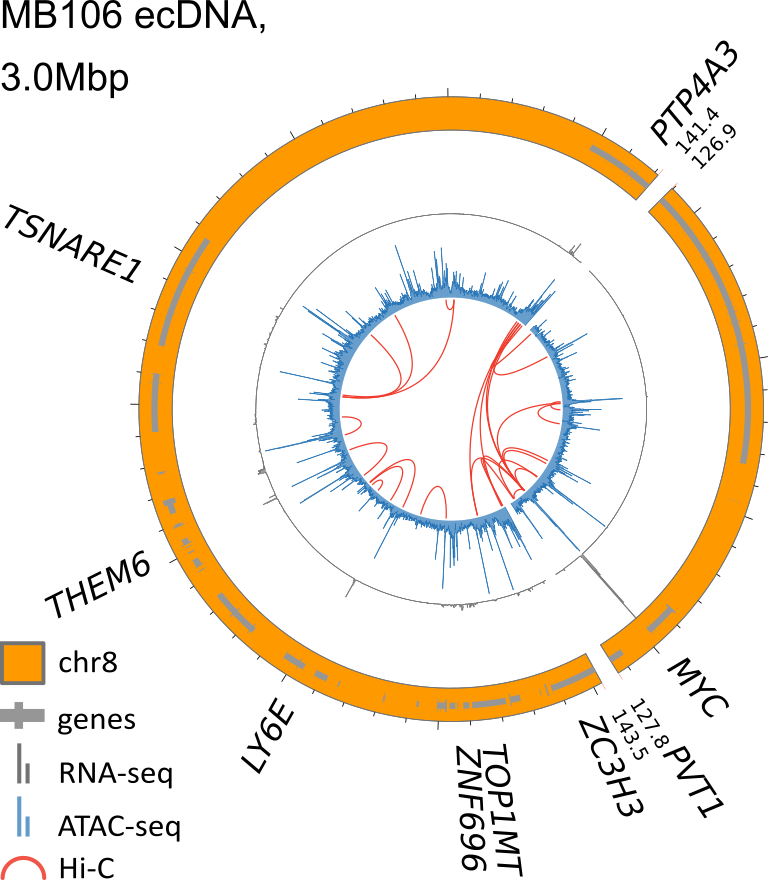
\includegraphics{MB106-circos}
        \caption{}
        \label{subfig:MB106-circos}
    \end{subfigure}
    \begin{subfigure}{.49\textwidth}
        \centering
        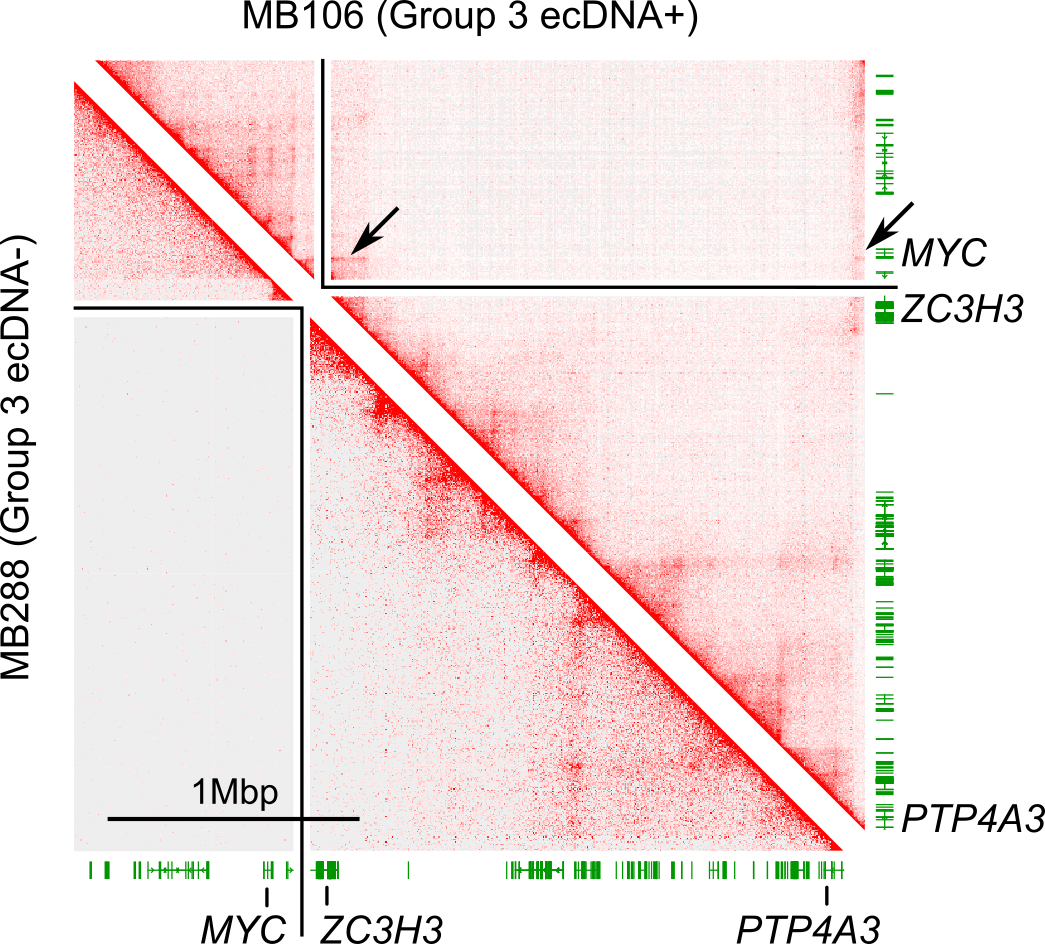
\includegraphics{MB106-MB288-ecDNA}
        \caption{}
        \label{subfig:MB106-MB288-hic}
    \end{subfigure}
    \caption[Transcriptional regulatory circuitry of ecDNA in \textit{MYC}-amplified Group 3 patient tumor MB106.]{\textbf{Transcriptional regulatory circuitry of ecDNA in \textit{MYC}-amplified Group 3 patient tumor MB106.} (\textbf{a}) Circular multi-omic map of the ecDNA sequence identified in Group 3 MB sample MB106. \textit{MYC} is highly expressed, and interacts with distal accessible loci located elsewhere on the ecDNA sequence. (\textbf{b}) Comparison of interaction densities at the MB106 ecDNA locus between MB106 (Group 3 ecDNA+) and MB288 (Group 3 ecDNA-). Ectopic interactions (arrows) between co-amplified segments of chr8 in MB106 are not present in the MB288 tumor with unrearranged \textit{MYC} locus.
    }
    \label{fig:MB106-MB288-myc-hic}
\end{figure}

In the SHH MB primary tumor MB268, we identified a 10.2Mbp ecDNA amplification which included the p53 regulator \textit{MDM4} \cite{toledo_2007} and is among the largest ecDNA amplifications identified in a patient tumor to date (Fig. \ref{fig:MB268}). \textit{MDM4} is recurrently amplified on glioblastoma ecDNA \cite{AA} and is a putative driver event in the MB268 tumor. On the same ecDNA, we also observed aberrant DNA interactions with the immune complement system regulator \textit{CFH} promoter. However, the functional significance of these co-amplified genes and DNA interactions remains unclear. 

\begin{figure}[!h]
    \centering
    \begin{subfigure}{.49\textwidth}
        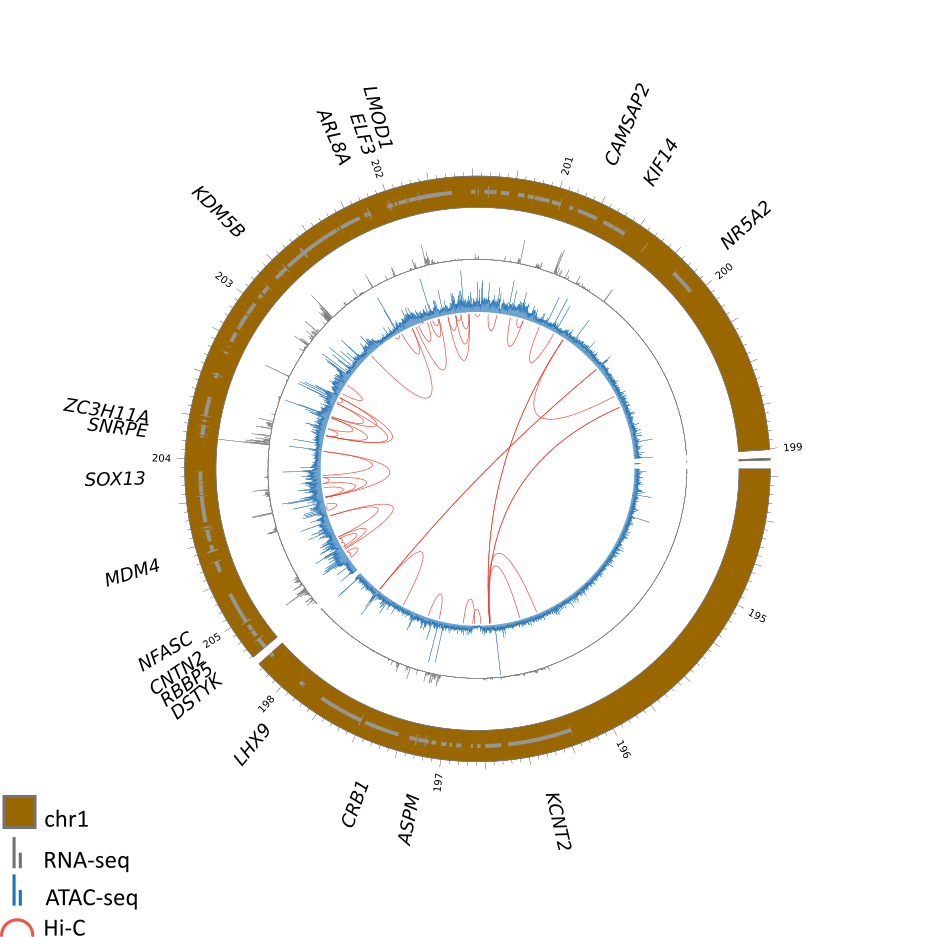
\includegraphics{MB268-circos}
    \end{subfigure}
    \begin{subfigure}{.49\textwidth}
        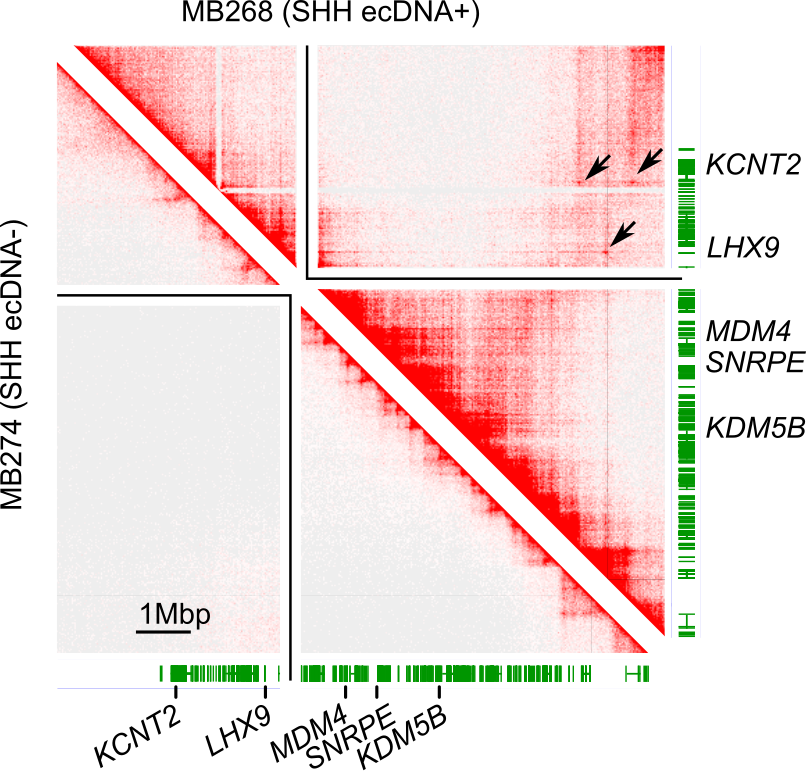
\includegraphics{MB268-hic}
    \end{subfigure}
    \caption[Transcriptional regulatory circuitry of ecDNA in SHH MB tumor MB268.]{\textbf{Transcriptional regulatory circuitry of ecDNA in SHH MB tumor MB268.} (\textbf{a}) Circular multi-omic map of the ecDNA present in the SHH MB patient tumor MB268. \textit{MDM4} is a negative p53 regulator recurrently amplified in glioblastoma \cite{AA}, and is a putative driver oncogene on this amplicon. (\textbf{b})Comparison of interaction densities at the MB268 ecDNA locus between MB268 (SHH ecDNA+) and MB274 (SHH ecDNA-). Ectopic interactions (arrows) between co-amplified segments of chr1 in MB268 are not present in unrearranged the MB274 tumor.
    }
    \label{fig:MB268}
\end{figure}

\par In two instances, the SHH MB tumor RCMB56-pdx and the Group 3 MB cell line D458, we identified rewired interactions between genomic loci originating from different chromosomes but co-amplified on the same ecDNA. As described above, RCMB56 harbored an ecDNA comprised of segments of chr1, and a complex extrachromosomal amplification comprised of segments of chr7 and chr17. Hi-C data indicated frequent chromatin interaction across breakpoints in each of the two amplicons present in this tumor (Fig. \ref{fig:RCMB56-circos}-\ref{fig:RCMB56-hic}). Aberrant chromatin interactions mapping to amp1 targeted accessible regions at the \textit{DNTTIP2}, \textit{SH3GLB1}, and \textit{SELENOF} gene loci (Fig. \ref{subfig:amp1-hic}). Aberrant interactions on amp2 included intrachromosomal interactions mapping to \textit{RPA3}, \textit{HERPUD2}, \textit{KLF14} and others; and trans-chromosomal interactions between the \textit{SP2} locus and the brain-specific long noncoding RNA \textit{LINC0301359}, and from the \textit{PRR15L} promoter to an intragenic region upstream of \textit{SRI} (Fig. \ref{subfig:amp2-hic}). 

\begin{figure}[!h]
    \centering
    \begin{subfigure}{.49\textwidth}
        \centering
        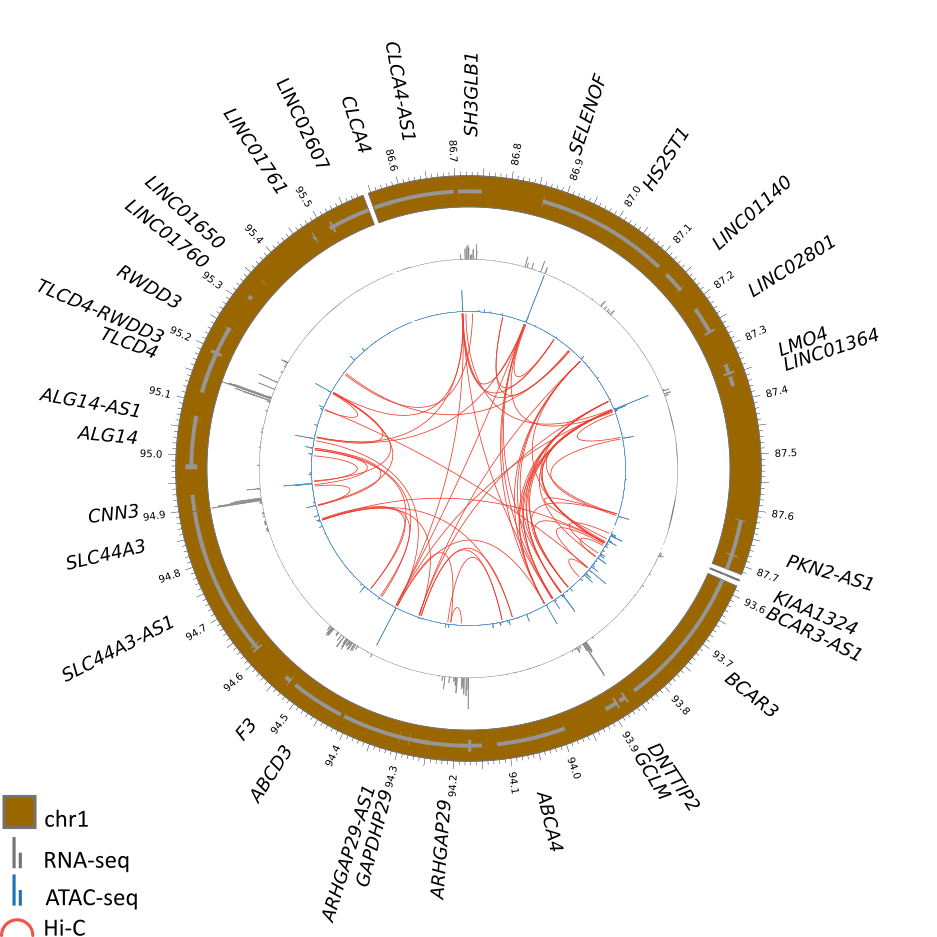
\includegraphics{RCMB56-amp1-circos}
        \caption{}
        \label{subfig:amp1-circos}
    \end{subfigure}
    \begin{subfigure}{.49\textwidth}
        \centering
        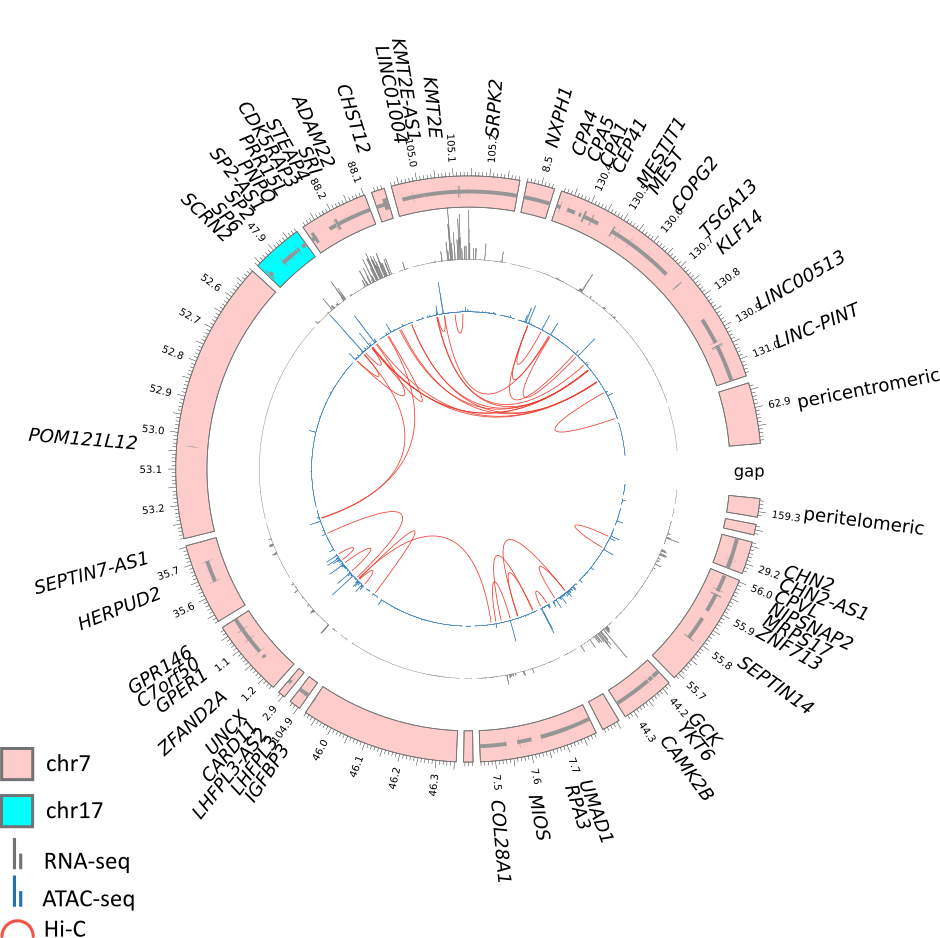
\includegraphics{RCMB56-amp2-circos}
        \caption{}
        \label{subfig:amp2-circos}
    \end{subfigure}
    \caption[Transcriptional regulatory circuitry of ecDNA sequences in RCMB56 p53-mutant SHH MB tumors.]{\textbf{Transcriptional regulatory circuitry of ecDNA sequences in RCMB56 p53-mutant SHH MB tumors.} (\textbf{a}) Transcription (RNA-seq, grey), accessible chromatin (blue), and chromatin interactions (Hi-C, red arcs) mapped onto the amp1 assembly (outer track, brown). Chromatin interactions occur across a structural breakpoint between accessible loci near highly-expressed genes such as \textit{DNTTIP2}. (\textbf{b}) Transcription, accessible chromatin, and chromatin interactions mapped onto the amp2 assembly. The gap in the assembly is adjacent to pericentromeric and peritelomeric loci. Ectopic interactions putatively target \textit{RPA3}, \textit{HERPUD2}, \textit{KLF14}, \textit{SP2}, and others.}
    \label{fig:RCMB56-circos}
\end{figure}
\begin{figure}
    \begin{subfigure}{\textwidth}
        \centering
        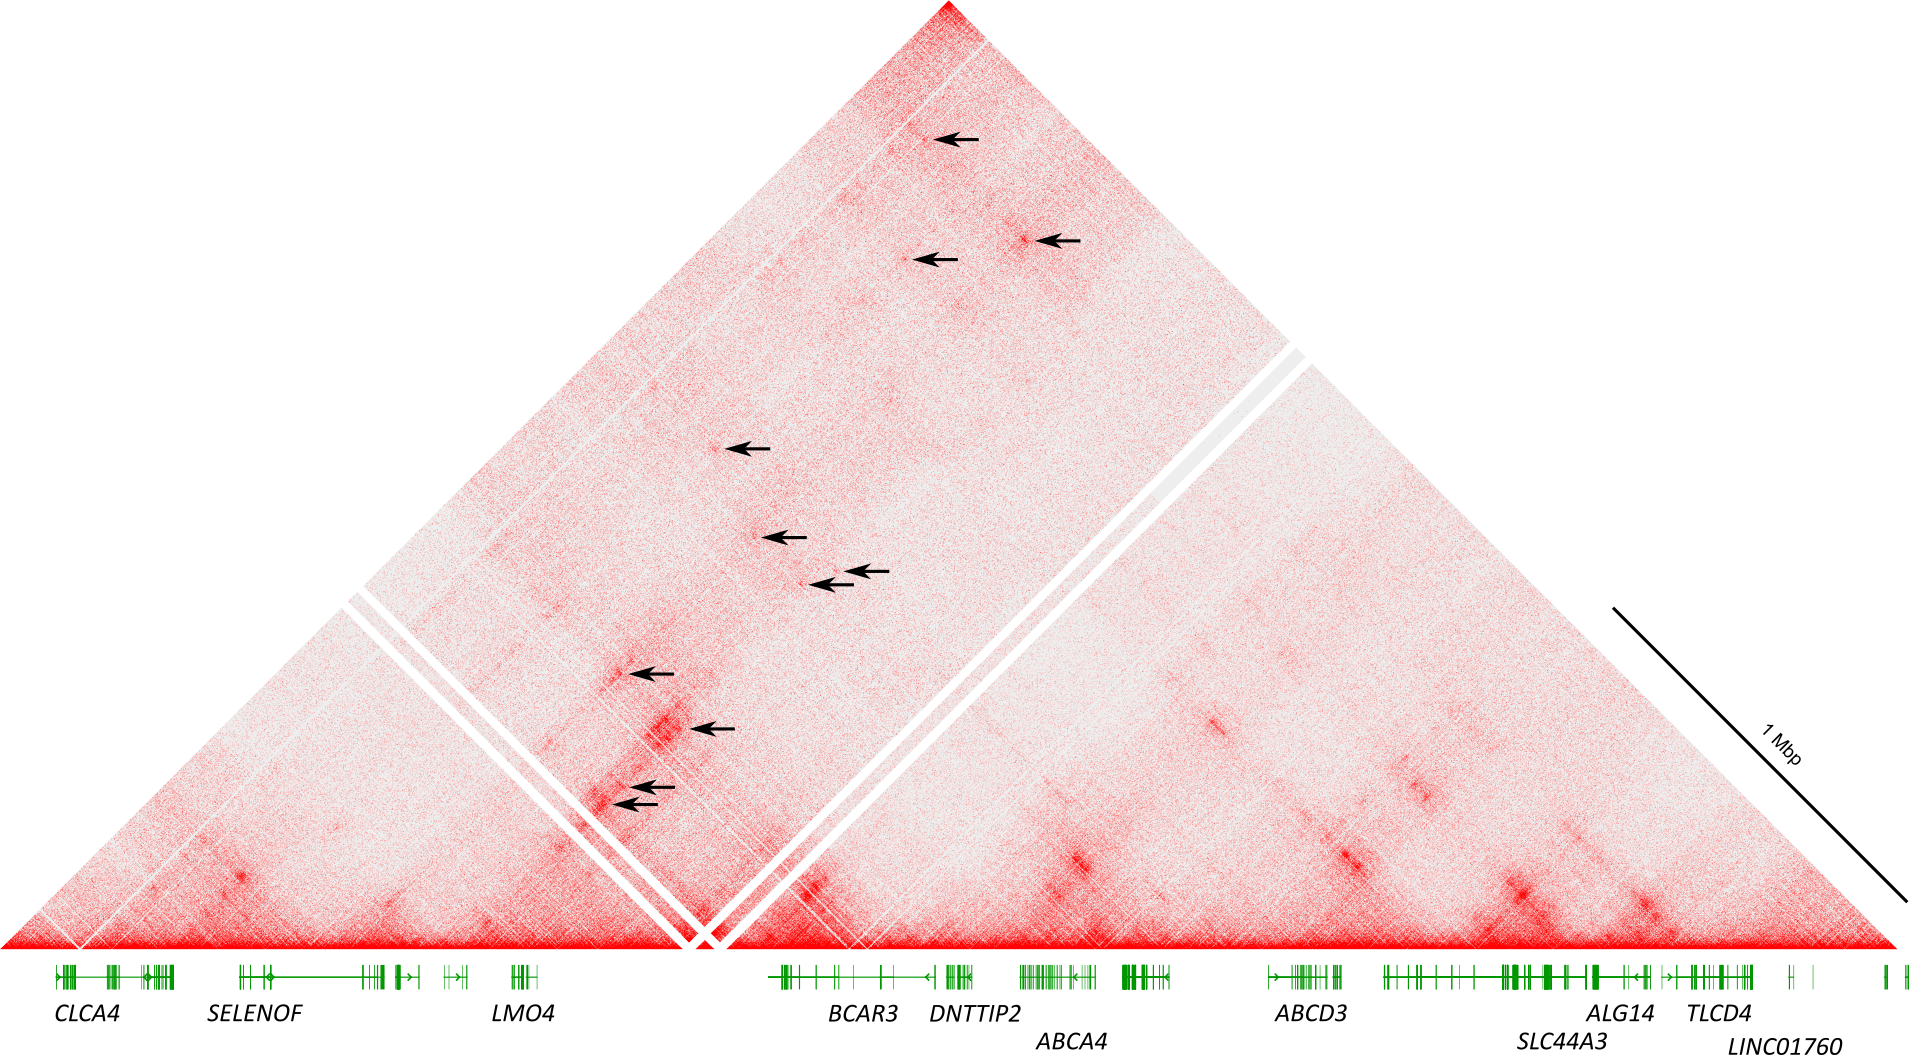
\includegraphics{RCMB56-amp1-hic}
        \caption{}
        \label{subfig:amp1-hic}
    \end{subfigure}
    \begin{subfigure}{\textwidth}
        \centering
        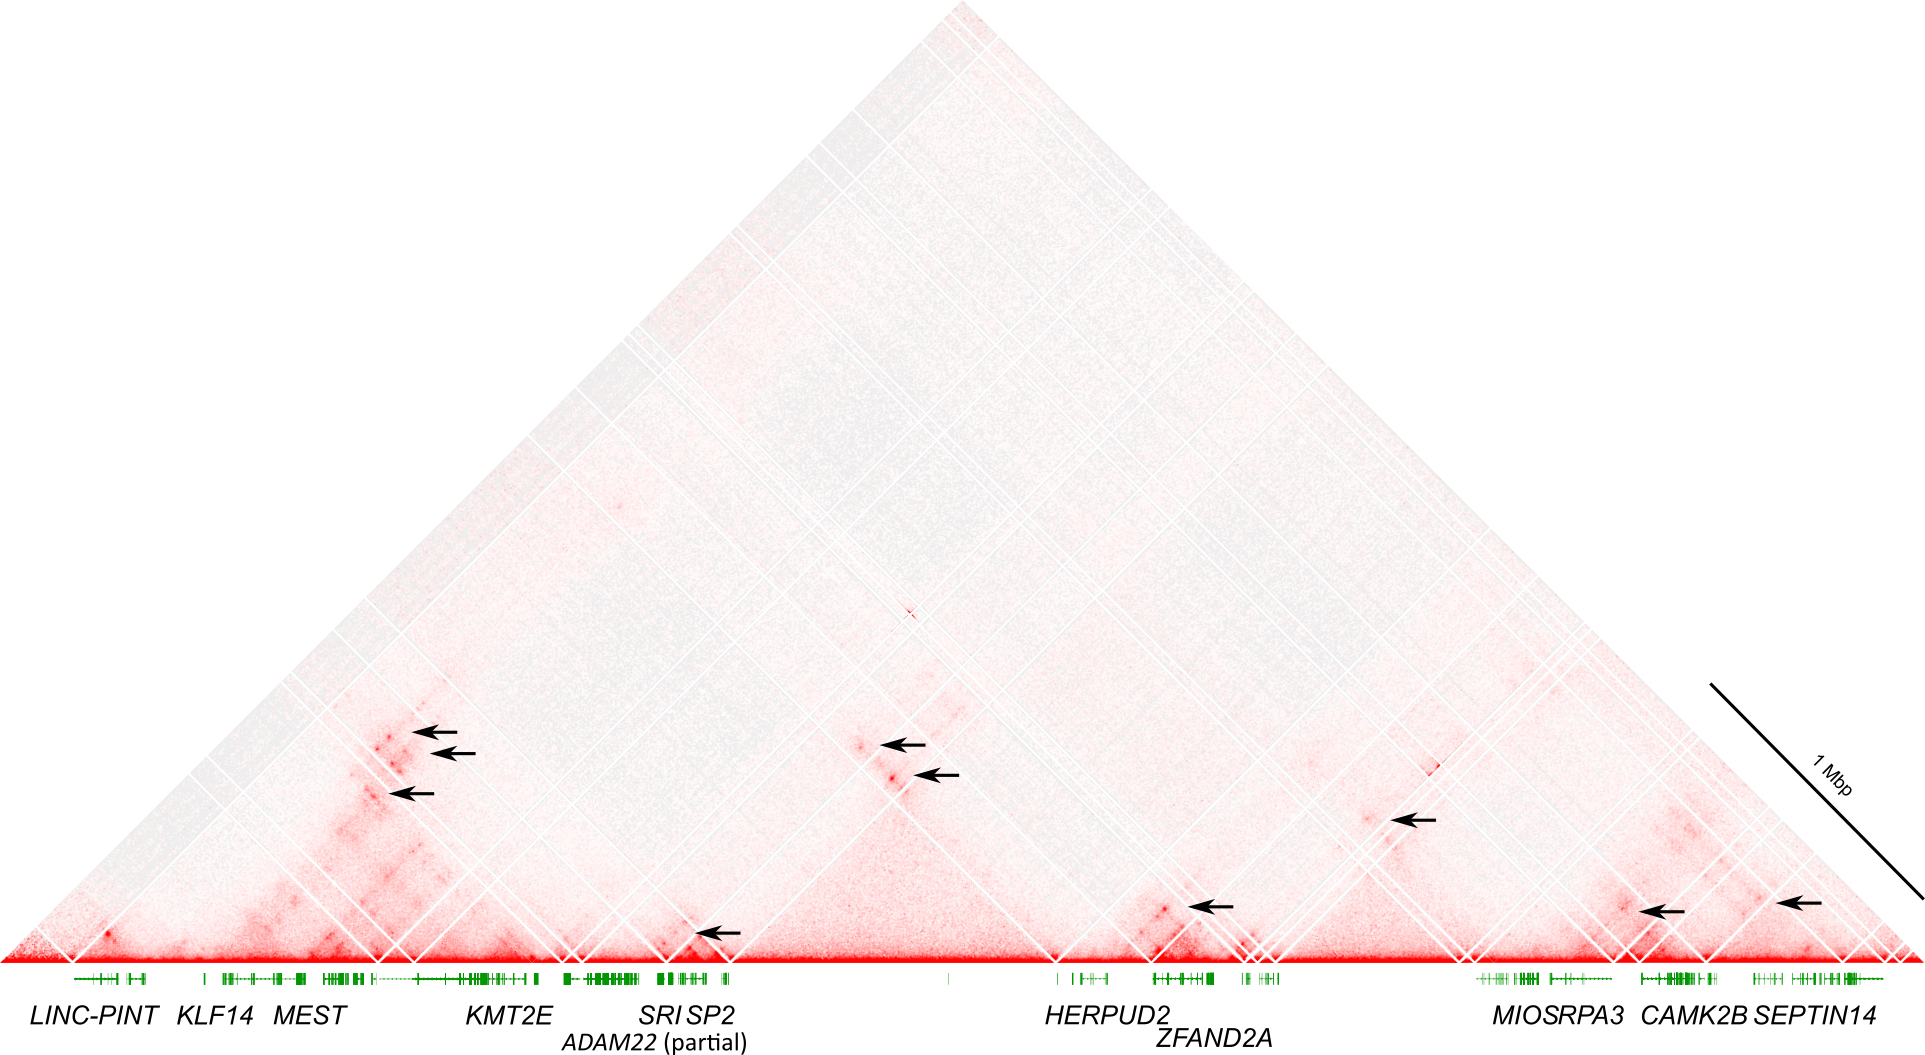
\includegraphics{RCMB56-amp2-hic}
        \caption{}
        \label{subfig:amp2-hic}
    \end{subfigure}
    \caption[Ectopic chromatin interactions on ecDNA in RCMB56.]{\textbf{Enhancer rewiring on ecDNA in RCMB56.} See also Fig. \ref{fig:RCMB56-circos}. (\textbf{a}) Chromatin interaction density map of the amp1 assembly. Arrows indicate putative enhancer rewiring events, or chromatin loops which span a breakpoint on the amp1 assembly. (\textbf{b}) Chromatin interaction density map of the amp2 assembly. Putative enhancer hijacking events are again indicated by arrows. The two ends of this assembly do not interact (top of the triangle), suggesting that they are spatially distant in the cell.}
    \label{fig:RCMB56-hic}
\end{figure}

\par D458 harbors an ecDNA amplification containing MB oncogenes \textit{MYC} and \textit{OTX2}, from chromosomes 8 and 14 respectively. Co-amplification of \textit{MYC} and \textit{OTX2} on the same ecDNA was validated by confocal FISH showing extrachromosomal co-localization of \textit{OTX2} and \textit{MYC} in D458 cells (Fig. \ref{D458-fish}), and by assembly of the D458 ecDNA from WGS and OGM data (Supplementary Fig. 11 of \cite{Chapman}). \textit{OTX2} is a known regulator of \textit{MYC} transcription and both genes are highly expressed in D458 (Fig. \ref{subfig:f4e}). The Hi-C data revealed several interactions of the \textit{MYC} promoter with co-amplified regulatory elements of chr8 and chr14 (Fig. \ref{fig:D458-ecDNA}). In summary, these results show that aberrant enhancer-promoter interactions resulting from structural rearrangements on ecDNA are common in MB tumors. 

\begin{figure}[!h]
    \centering
    \begin{subfigure}{\textwidth}
        \centering
        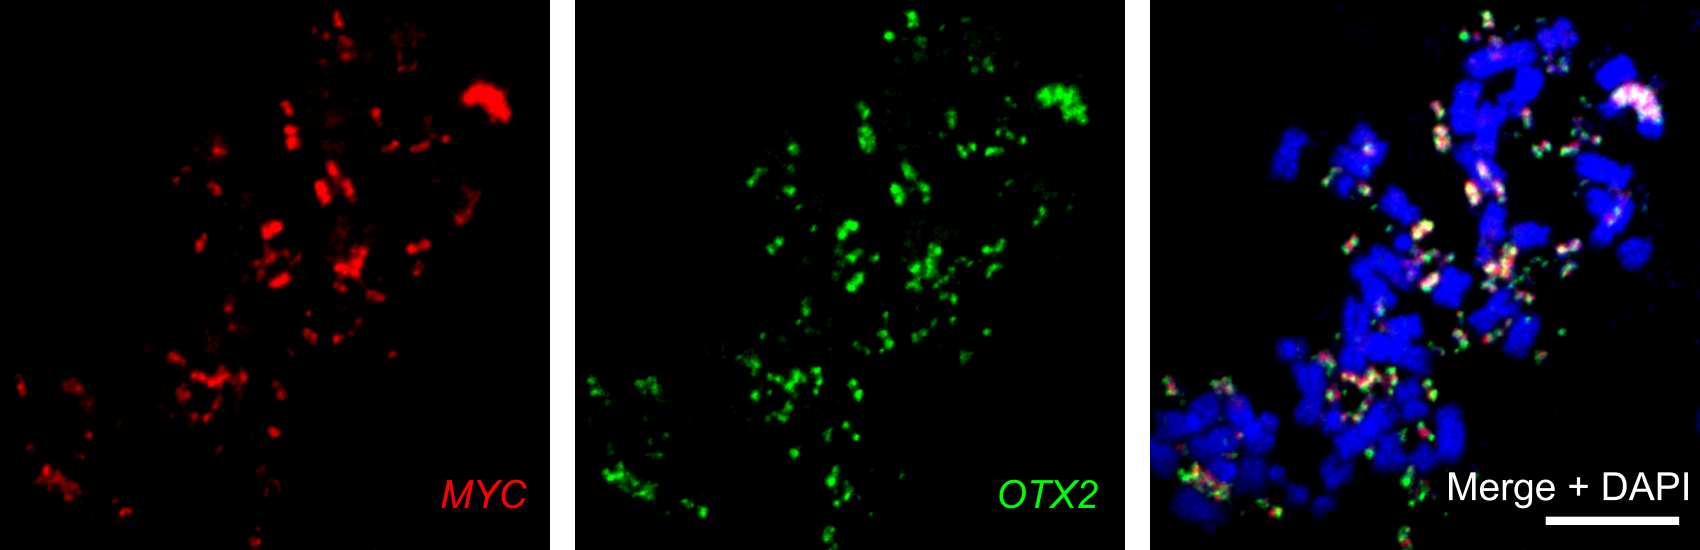
\includegraphics{D458-fish}
        \caption{}
        \label{D458-fish}
    \end{subfigure}
    \begin{subfigure}{.54\textwidth}
        \centering
        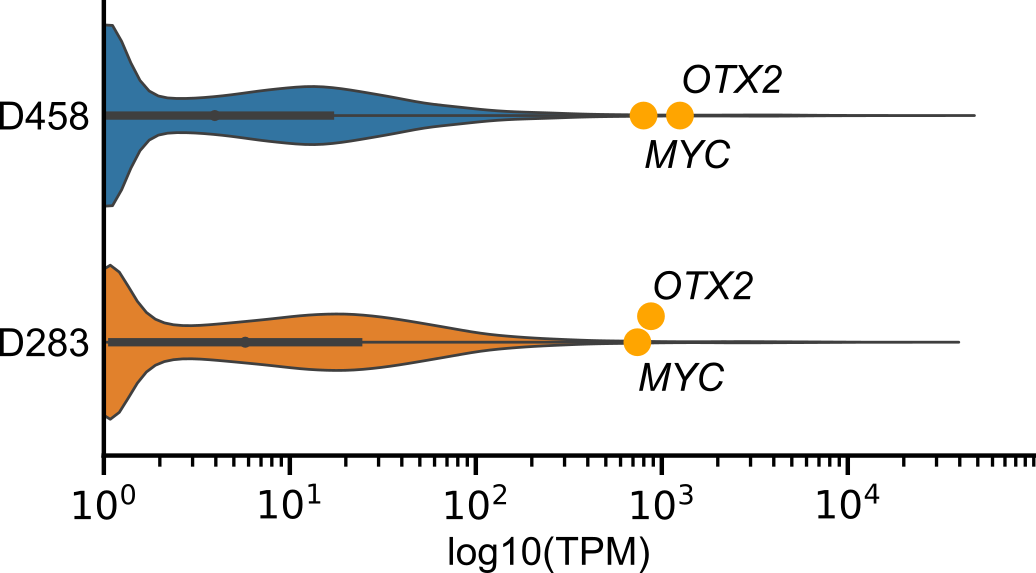
\includegraphics[right]{f4e}
        \caption{}
        \label{subfig:f4e}
    \end{subfigure}
    \begin{subfigure}{.44\textwidth}
        \centering
        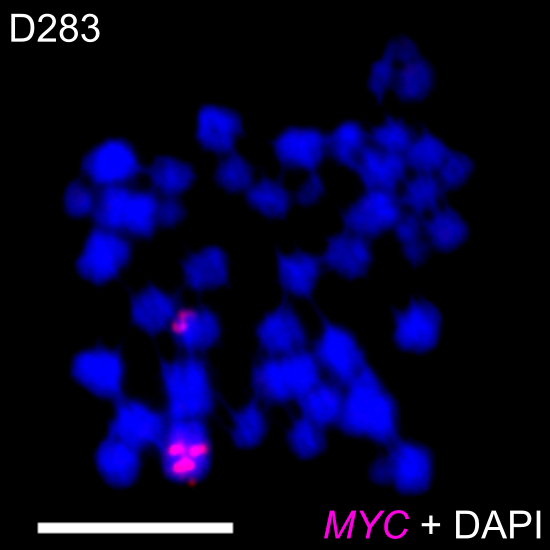
\includegraphics[right=2cm]{D283-fish}
        \caption{}
        \label{subfig:D283-fish}
    \end{subfigure}
    \caption[Two Group 3 MB cell lines with intra- and extrachromosomal \textit{MYC} amplifications.]{\textbf{Two Group 3 MB cell lines with intra- and extrachromosomal \textit{MYC} amplifications.} (\textbf{a}) Confocal FISH of \textit{MYC} and \textit{OTX2} on a metaphase spread of a D458 cell. (\textbf{b}) Gene transcription of all protein-coding genes in D458 and D283 from publicly available data in DepMap \cite{depmap}.  MB Group 3 oncogenes \textit{MYC} and \textit{OTX2} are highlighted. (\textbf{c}) FISH in a metaphase spread of a D283 nucleus shows chromosomal \gls{HSR} \textit{MYC} amplification. \textit{OTX2} is not amplified in D283.}
    \label{fig:D458-fish}
\end{figure}

\begin{figure}[!h]
    \begin{subfigure}{\textwidth}
        \centering
        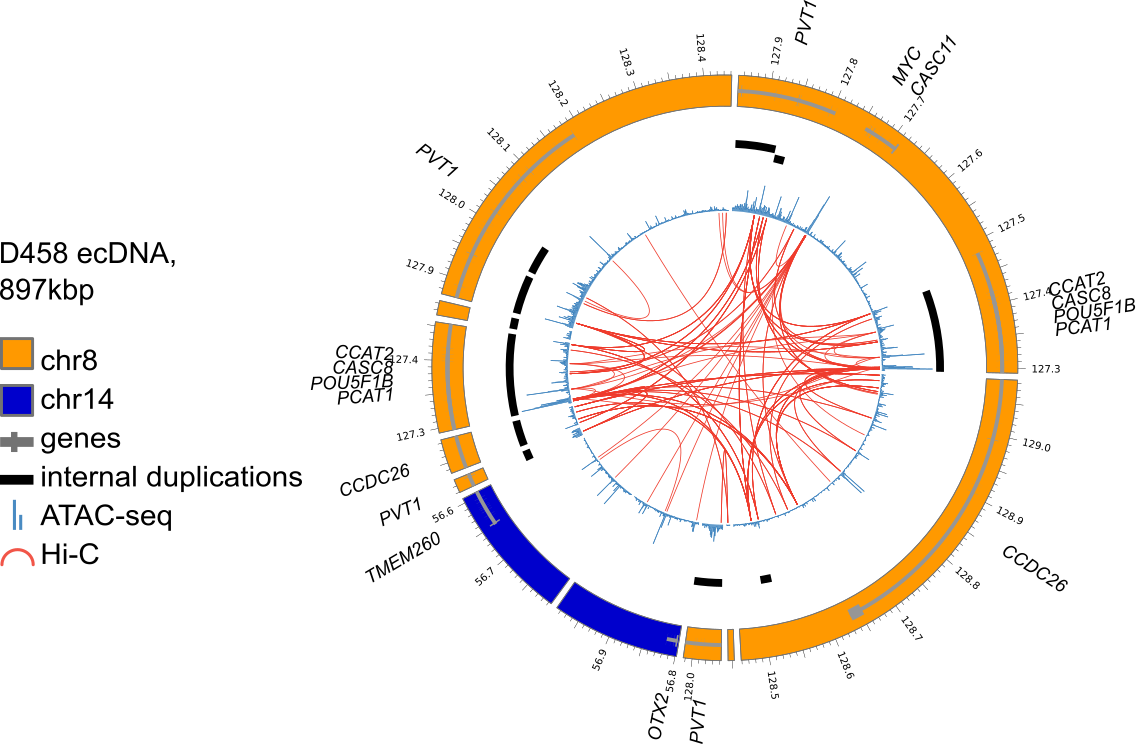
\includegraphics{D458-circos}
        \caption{}
        \label{subfig:D458-circos}
    \end{subfigure}
    \begin{subfigure}{\textwidth}
        \centering
        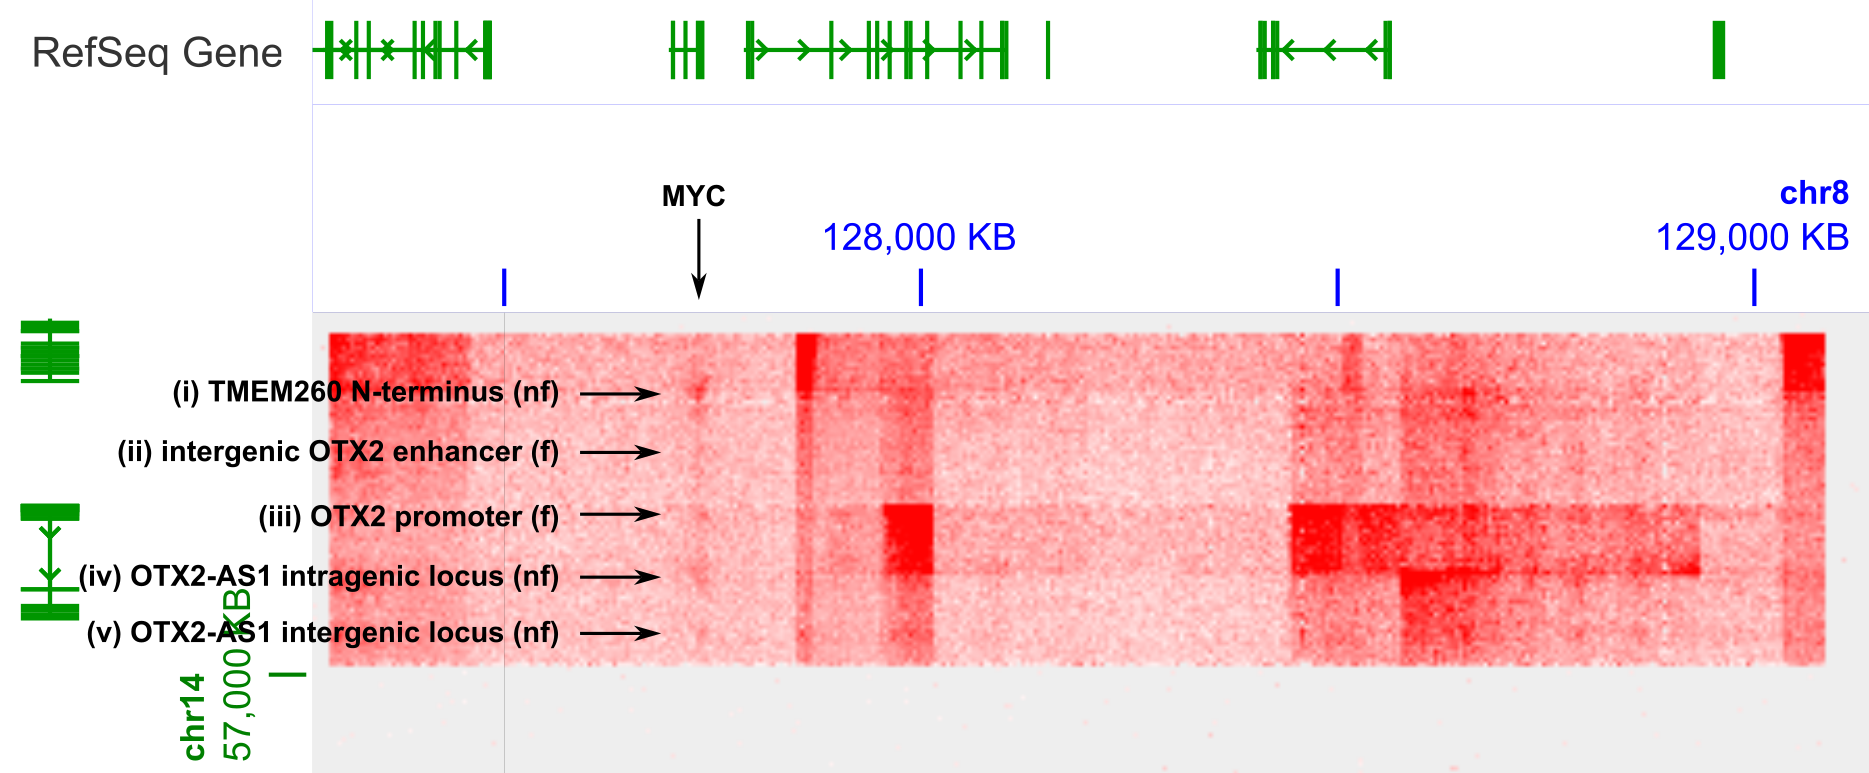
\includegraphics{D458-hic}
        \caption{}
        \label{subfig:D458-hic}
    \end{subfigure}
    \caption[Transcriptional regulatory map of the D458 ecDNA.]{\textbf{Transcriptional regulatory map of the D458 ecDNA.} (\textbf{a}) Circular map of accessible chromatin (blue) and chromatin interactions (red) mapping to the D458 ecDNA sequence assembly. 
    (\textbf{b}) Interchromosomal interactions between segments of the D458 ecDNA originating from chr8 and chr14. Arrows highlight putative chromatin loops included in (a). f: functional, as determined by a significant and D458-specific effect on cell proliferation upon CRISPRi inhibition (Fig. \ref{fig:crispri-pooled}); nf: not identified as functional in the same pooled CRISPRi screen.
    }
    \label{fig:D458-ecDNA}
\end{figure}

\subsection{Co-amplified enhancers shape the transcriptional regulatory circuitry of ecDNA.}
To test whether the observed enhancer rewiring events in ecDNA have functional roles in tumor cell proliferation, we performed a pooled CRISPRi proliferation screen in the Group 3 MB cell line D458, targeting all 645 accessible loci co-amplified on the ecDNA using 32,530 small guide RNA sequences (sgRNAs). These loci included 10 highly accessible regions from chr14, each overlapping ENCODE candidate cis-regulatory elements (cCREs) \cite{encode}. Because enhancer usage is highly conserved in Group 3 MB tumors \cite{lin_2017}, we performed the same screen in the Group 3 cell line D283, in which \textit{MYC} (but not \textit{OTX2}) is tandem amplified on a 55Mbp \gls{HSR} of chr8q (Fig. \ref{subfig:D283-fish}). While the \textit{MYC} promoter was essential in both cell lines, our screen identified 6 functional elements which, upon CRISPRi inhibition, specifically reduced D458 proliferation compared to D283 after 21 days (MAGeCK MLE, $q < 0.05$; Fig. \ref{fig:crispri-pooled}) \cite{mageck}. On chr8, these loci included two accessible regions of a known \textit{MYC} superenhancer \cite{lin_2017} and the \textit{PVT1} promoter. In D458, much of the superenhancer is duplicated internally on the ecDNA, and \textit{PVT1} is amplified in D458 but not in D283.  Conversely, we observed that other accessible regions of the same \textit{MYC} superenhancer were specifically essential for D283 but not for D458, indicating altered regulatory dependencies on the \textit{MYC}-ecDNA compared to the \textit{MYC}-HSR amplification. These results are consistent with a previous comparison of ecDNA+ and ecDNA- glioblastoma cell lines, where the impact of enhancer silencing on proliferation was associated with cell line-specific chromatin accessibility and interactions \cite{Morton_2019}.

The Hi-C data indicated interactions between \textit{MYC} on chr8 and regulatory elements of chr14 co-amplified on the same ecDNA, two of which are essential for D458 proliferation (Fig. \ref{subfig:D458-hic}): a cluster of elements at the \textit{OTX2} locus as well as a distal enhancer \cite{wortham_2014} located 80kbp downstream of \textit{OTX2} on the reference genome, but inverted on the ecDNA. D283-specific elements on chr14 included peaks at the N-terminal exon of \textit{OTX2} and another distal enhancer \cite{wortham_2014} 55kbp from \textit{OTX2} on the reference but also inverted on the ecDNA. To further test the influence on transcription of regulatory regions essential in D458 but not in D283, we performed additional CRISPRi inhibition experiments targeted against the \textit{PVT1} promoter and an accessible region within the internal duplication of the \textit{MYC} superenhancer. Consistent with the result of the CRIPSRi proliferation screen, silencing of the \textit{MYC} superenhancer reduced \textit{MYC} expression for 2 out of 3 tested sgRNAs in D458 but not in D283 (Fig. \ref{fig:crispri-myc-se}). No significant difference was observed in \textit{OTX2} transcription in either cell line. Silencing of the \textit{PVT1} promoter abrogated \textit{PVT1} transcription but not \textit{MYC} or \textit{OTX2}, in D458 but not in D283 (Fig. \ref{fig:crispri-pvt1-tss}). Thus, although proliferation in both Group 3 MB cell lines is driven by \textit{MYC} amplification, the relative importance of co-amplified genes and cis-regulatory elements is specific to the genomic architecture of the amplicon.

% Pooled CRISPRi screen
\begin{figure}[!h]
    \centering
    \centerline{%
    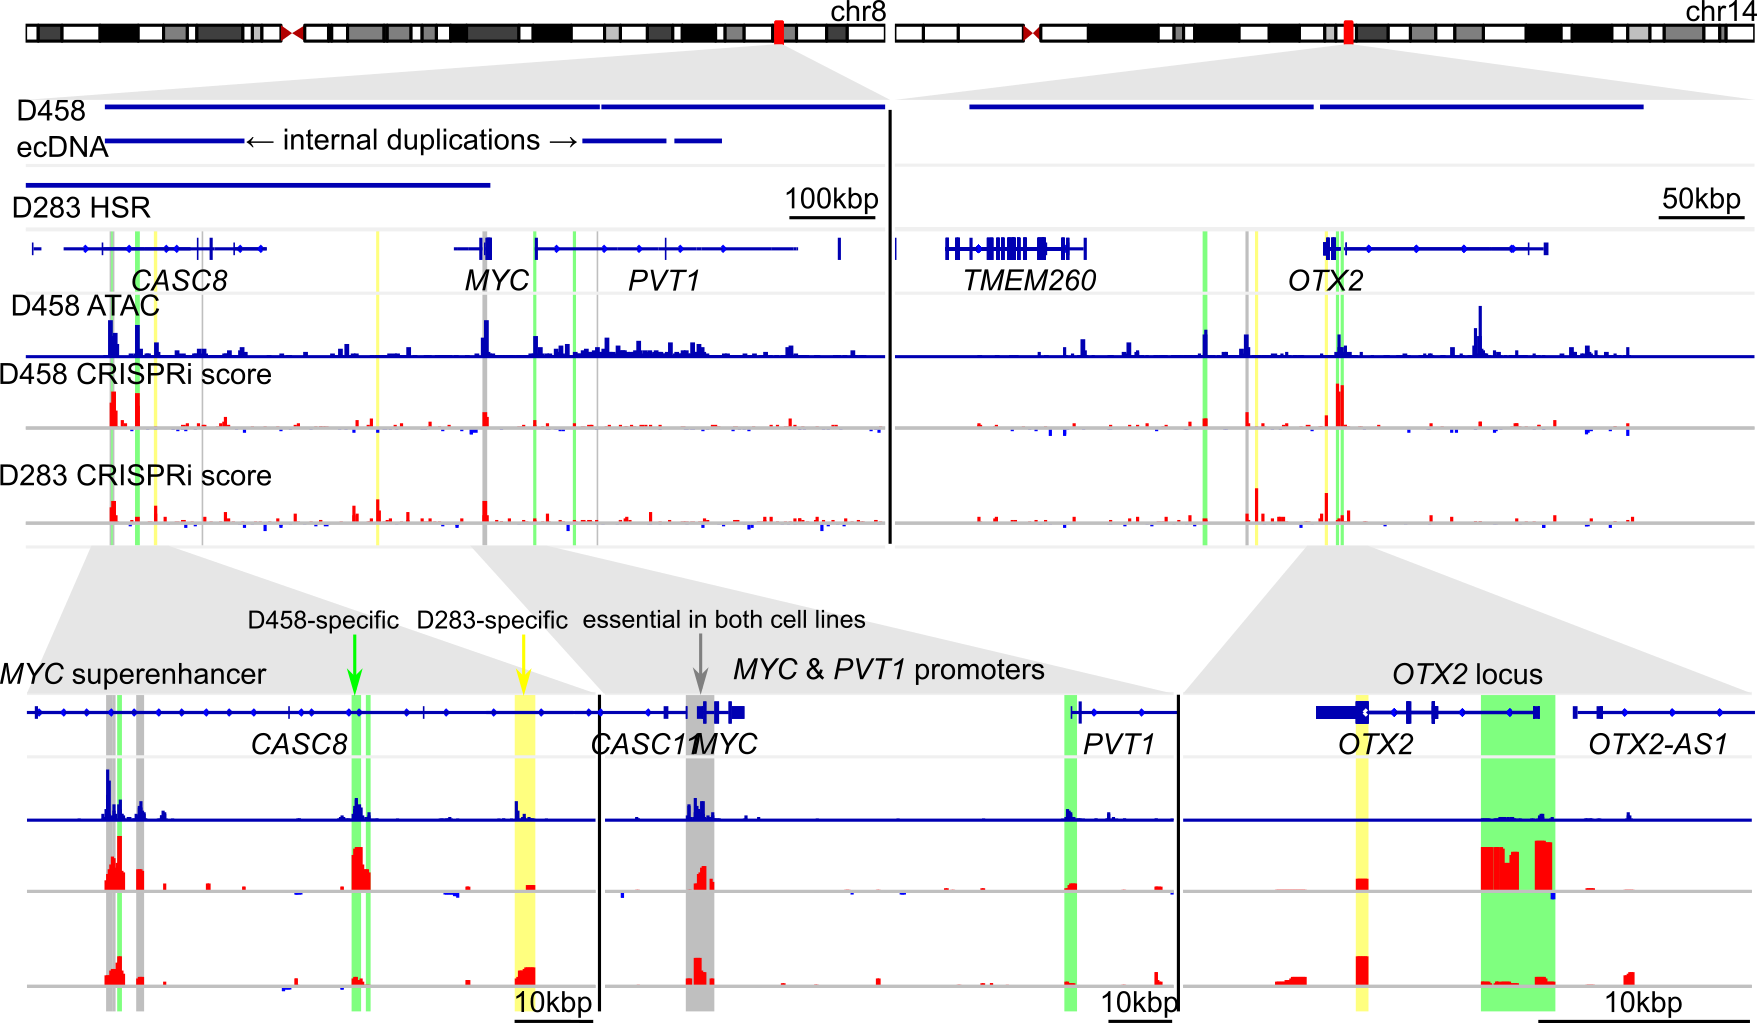
\includegraphics{pooled-screen}%
    }
    \caption[A large CRISPRi screen identifies differentially active enhancers in two \textit{MYC} amplicons.]{\textbf{A large CRISPRi screen identifies differentially active enhancers in two \textit{MYC} amplicons.} Pooled CRISPRi screen in the two G3 MB cell lines D458 (\textit{MYC} ecDNA) and D283 (\textit{MYC} HSR) targeted against all accessible loci on the D458 ecDNA as identified by ATAC-seq. Tracks from top to bottom: amplified regions of the D458 ecDNA; amplified regions of the D283 HSR; refSeq genes; D458 bulk ATAC-seq signal; CRISPRi essentiality score tracks for D458 and D283 generated by CRISPR-SURF \cite{crispr-surf}. Vertical highlighted bars indicate accessible loci which are significantly depleted at T21 relative to T0, and colored by cell line specificity. Grey: essential in D458 and D283 with no significant difference; green: significantly depleted in D458 relative to D283; yellow: significantly depleted in D283 relative to D458. All significance values determined by FDR-corrected MAGeCK-MLE permutation test \cite{mageck} ($q < 0.05$).}
    \label{fig:crispri-pooled}
\end{figure}

% Targeted CRISPRi of MYC SE
\begin{figure}[!h]
    \centering
    \begin{subfigure}{.49\textwidth}
        \centering
        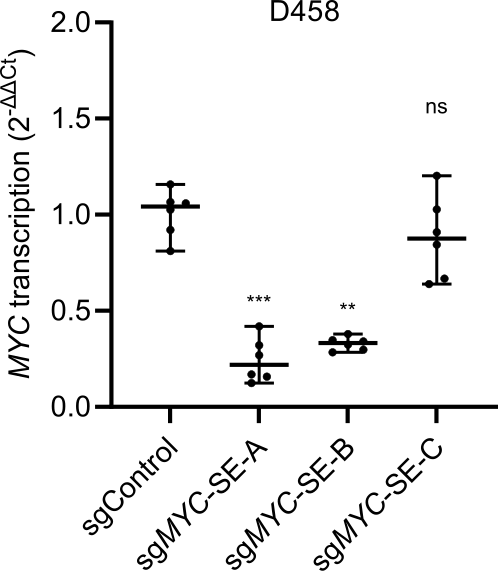
\includegraphics{D458-MYC-SE-MYC}
        \caption{}
        \label{subfig:d458-myc-se-myc}
    \end{subfigure}
    \begin{subfigure}{.49\textwidth}
        \centering
        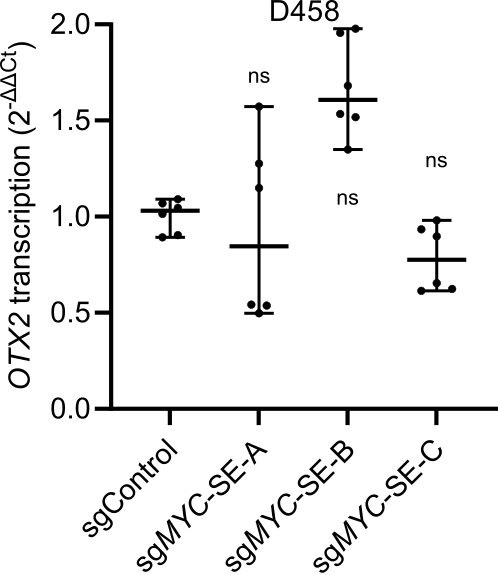
\includegraphics{D458-MYC-SE-OTX2}
        \caption{}
        \label{subfig:d458-myc-se-otx2}
    \end{subfigure}
    \begin{subfigure}{.49\textwidth}
        \centering
        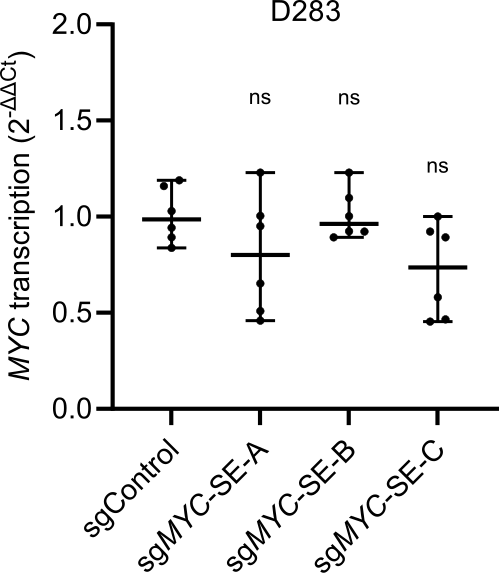
\includegraphics{D283-MYC-SE-MYC}
        \caption{}
        \label{subfig:d283-myc-se-myc}
    \end{subfigure}
    \begin{subfigure}{.49\textwidth}
        \centering
        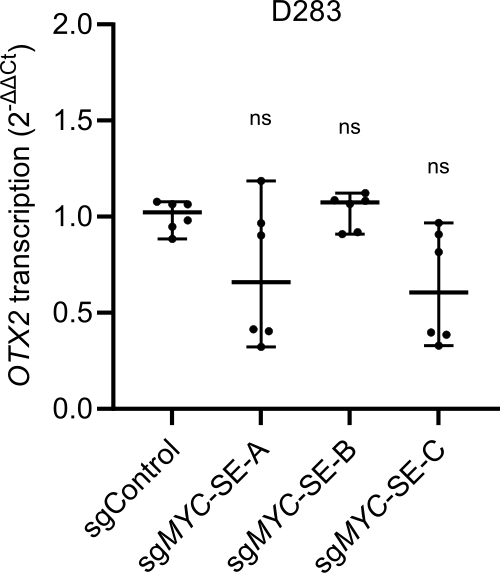
\includegraphics{D283-MYC-SE-OTX2}
        \caption{}
        \label{subfig:d283-myc-se-otx2}
    \end{subfigure}
    \caption[A co-amplified enhancer on the D458 ecDNA promotes \textit{MYC} expression.]{\textbf{A co-amplified enhancer on the D458 ecDNA promotes \textit{MYC} expression.} Relative expression of \textit{MYC} and \textit{OTX2} in D458 (\textbf{a}-\textbf{b}) and D283 (\textbf{c}-\textbf{d}), measured by qPCR ($2^{-\Delta\Delta Ct}$), in D458 and D283 cell lines upon CRISPRi targeting of an accessible locus within a known \textit{MYC} superenhancer which promotes D458 proliferation (see also Fig. \ref{fig:crispri-pooled}). sgNT: nontargeting control; sg\textit{MYC}-SE-A-C: sgRNAs targeting the \textit{MYC} enhancer at D458\_peak\_30782, positions chr8:127330655, chr8:127330840, and chr8:127330927 respectively. qPCR was performed on all guides in technical triplicate. All co-ordinates refer to the hg38 assembly. ** $p < 0.01$; *** $p < 0.001$; nested ANOVA with Dunnett’s correction.
    }
    \label{fig:crispri-myc-se}
\end{figure}

% Targeted CRISPRi of PVT1 TSS
\begin{figure}[!h]
    \centering
    \begin{subfigure}{.32\textwidth}
        \centering
        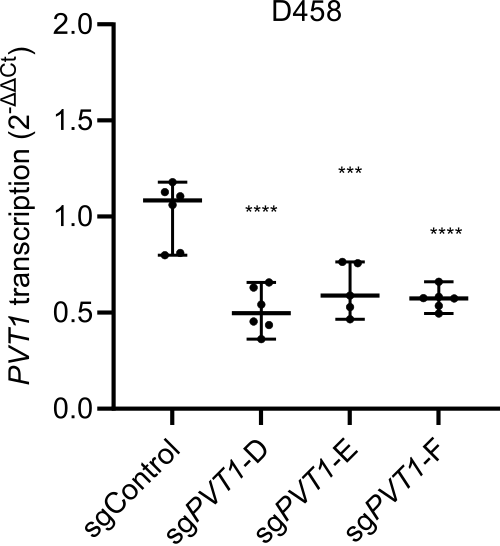
\includegraphics{D458-PVT1-TSS-PVT1}
        \caption{}
        \label{subfig:d458-pvt1-tss-pvt1}
    \end{subfigure}
    \begin{subfigure}{.32\textwidth}
        \centering
        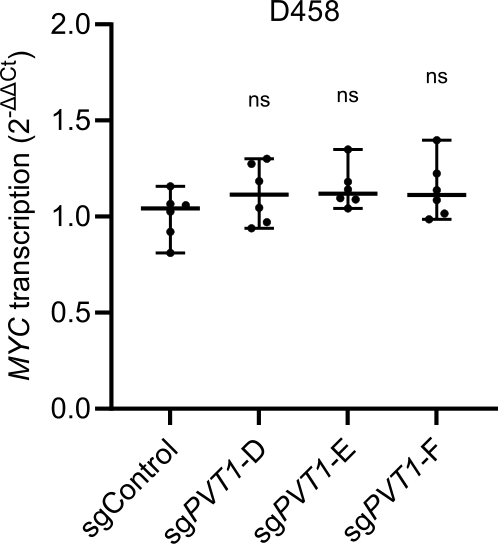
\includegraphics{D458-PVT1-TSS-MYC}
        \caption{}
        \label{subfig:d458-pvt1-tss-myc}
    \end{subfigure}
    \begin{subfigure}{.32\textwidth}
        \centering
        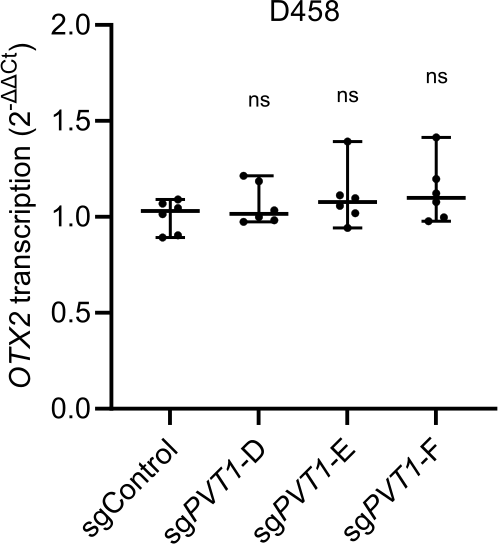
\includegraphics{D458-PVT1-TSS-OTX2}
        \caption{}
        \label{subfig:d458-pvt1-tss-otx2}
    \end{subfigure}
    \begin{subfigure}{.32\textwidth}
        \centering
        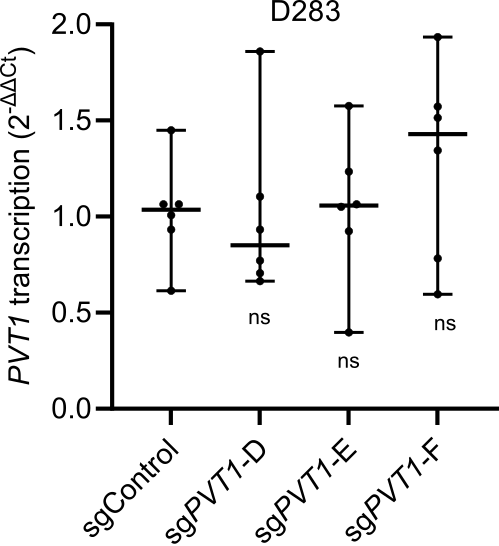
\includegraphics{D283-PVT1-TSS-PVT1}
        \caption{}
        \label{subfig:d283-pvt1-tss-pvt1}
    \end{subfigure}
    \begin{subfigure}{.32\textwidth}
        \centering
        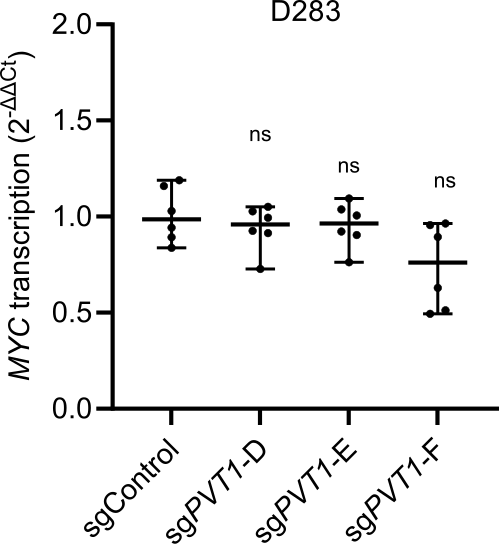
\includegraphics{D283-PVT1-TSS-MYC}
        \caption{}
        \label{subfig:d283-pvt1-tss-myc}
    \end{subfigure}
    \begin{subfigure}{.32\textwidth}
        \centering
        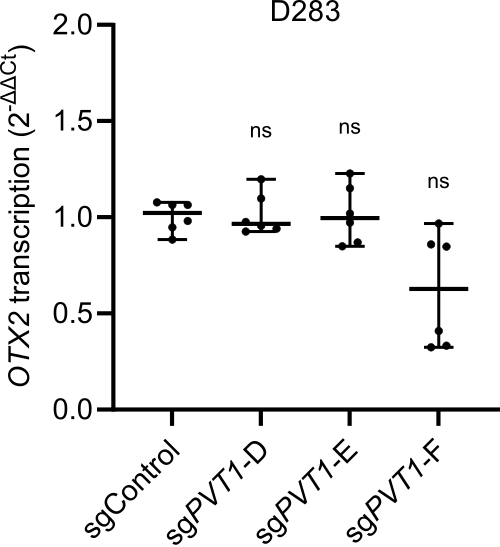
\includegraphics{D283-PVT1-TSS-OTX2}
        \caption{}
        \label{subfig:d283-pvt1-tss-otx2}
    \end{subfigure}
    \caption[\textit{PVT1} promotes D458 cell proliferation.]{\textbf{\textit{PVT1} promotes D458 cell proliferation.} 
     Relative expression of \textit{PVT1}, \textit{MYC}, and \textit{OTX2}, measured by qPCR ($2^{-\Delta\Delta Ct}$), in D458 (\textbf{a}-\textbf{c}) and D283 (\textbf{d}-\textbf{f}) cell lines upon CRISPRi targeting of the \textit{PVT1} promoter which promotes D458 proliferation (see also Fig. \ref{fig:crispri-pooled}). sgNT: nontargeting control; sg\textit{PVT1}-D-F: sgRNAs targeting the \textit{PVT1} promoter at D458\_peak\_30920, positions chr8:127794266, chr8:127794773, and chr8:127794945 respectively. qPCR was performed on all guides in triplicate. All co-ordinates refer to the hg38 assembly. *** $p < 0.001$; **** $p < 0.0001$; nested ANOVA with Dunnett’s correction.
    }
    \label{fig:crispri-pvt1-tss}
\end{figure}

\subsection{ecDNA interacts with chromosomal oncogene loci.}
Recent studies have revealed intermolecular enhancer-promoter interactions between ecDNA molecules (`ecDNA hubs') \cite{hung_2021} or between the chromosomes and ecDNA (`mobile enhancers') \cite{Zhu_2021}. To test for such intermolecular chromatin interactions in medulloblastoma, we computationally identified interchromosomal loops from Hi-C of the SHH MB tumor RCMB56-pdx, where one loop anchor mapped to the circular ecDNA amp1. This analysis revealed a nexus of interactions mapping from the \textit{ARHGAP29} locus on amp1 to loci elsewhere in the genome with plausible tumorigenic roles, including \textit{MECOM}, \textit{RAD51AP2}, \textit{POU4F1}, and \textit{IGF1R} (Fig. \ref{fig:mobile-enhancers}). However, the functional significance of these intermolecular chromatin interactions in MB remains untested.

% mobile enhancers
\begin{figure}[!h]
    \begin{subfigure}{.49\textwidth}
        \centering
        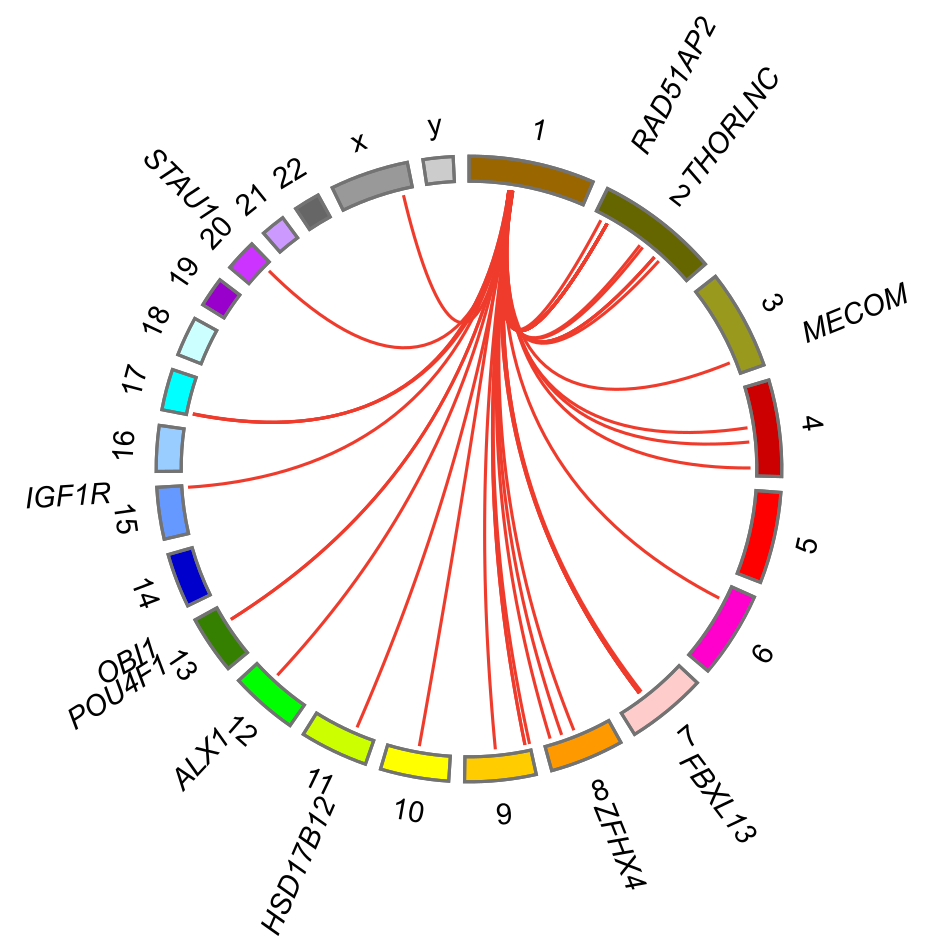
\includegraphics{RCMB56-amp1-trans-circos}
        \caption{}
        \label{subfig:RCMB56-amp1-trans}
    \end{subfigure}
    \begin{subfigure}{.49\textwidth}
        \centering
        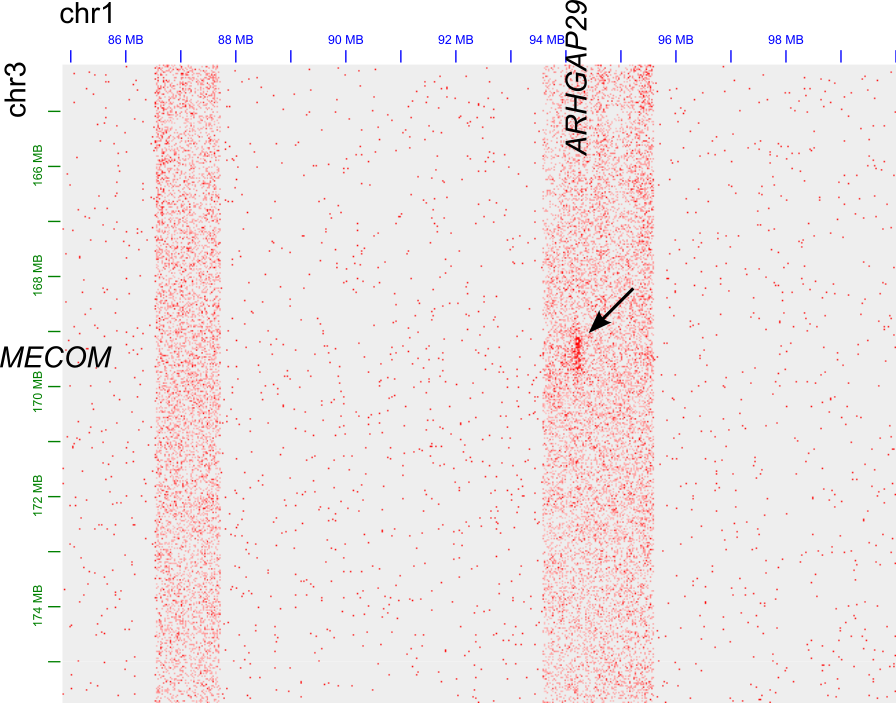
\includegraphics{RCMB56-amp1-trans-hic}
        \caption{}
        \label{subfig:rcmb56-mecom}
    \end{subfigure}
    \caption[The RCMB56 amp1 ecDNA interacts with chromosomal gene loci.]{\textbf{The RCMB56 amp1 ecDNA interacts with chromosomal gene loci.} (\textbf{a}) Interchromosomal chromatin interactions detected by FitHiC2 \cite{fithic2} between amp1 and other chromosomes. Interactions mapping to a gene locus are labelled. (\textbf{b})  Interaction density map between segments of chr1 and chr3, rendered in Juicebox \cite{juicebox}. Vertical stripes indicate increased contact density between the ecDNA and chr3 over background interactions between chr1 and chr3. Arrow indicates the chromatin loop detected between \textit{ARHGAP29} on amp1 and \textit{MECOM} on chr3. 
    }
    \label{fig:mobile-enhancers}
\end{figure}

\section{Discussion}
    
By mapping chromatin interactions occurring on ecDNA in patient and model tumors, we observe ectopic chromatin interactions occurring between genomic loci which are distal on the reference genome but proximal on the ecDNA. In representative tumors of the SHH and Group 3 \gls{MB} subgroups, these interactions targeted known or putative oncogene loci, and coincided with high gene expression. To determine the extent to which the enhancer landscape of an ecDNA may affect cell proliferation, we performed pooled and targeted CRISPR inhibition experiments in the Group 3 MB cell line D458, which amplifies oncogenes \textit{MYC}, \textit{OTX2}, and \textit{PVT1} on ecDNA. These experiments reveal that a distal \textit{MYC} superenhancer is essential to cell proliferation, and that the relative importance of specific enhancer sub-elements is specific to the sequence of the structural rearrangement. In this illustrative model, the rearranged enhancer landscape of the ecDNA sequence contributes to the cell's proliferative capacity.

Therapeutic targeting of rewired enhancers in patient tumors remains a major unresolved challenge. In our example Group 3 \textit{MYC}-amplified cell lines D283 and D458, the bromodomain inhibitor JQ1 attenuates cell growth by downregulating \textit{MYC} transcription \cite{bandopadhayay_2014}. The mechanism of action is believed to be disruption of BRD4-mediated binding of transcriptional machinery to \textit{MYC} enhancers, downregulating \textit{MYC} expression. However, clinical trials of BRD inhibitors have so far shown high rates of adverse events and limited efficacy \cite{sun_2020}. In addition, further research will be required to resolve and target the exact oncogenic seuqences driving patient tumors such as RCMB56, which does not amplify a known MB oncogene on either ecDNA amplification.

\section{Methods}
\subsection{ATAC-seq}
Archer \textit{et al.} samples. At least 25mg of pulverized frozen tissue from samples previously included in proteomics analysis5 were sequenced by ATAC-seq according to an established protocol for bulk ATAC-seq of frozen neuronal cells\cite{milani_2016}. Reads were aligned, deduplicated and preprocessed according to ENCODE best practices. Samples included in subsequent analyses passed the following quality control thresholds: PCR bottleneck coefficient 1 (PBC1) $> 0.7$, PCR bottleneck coefficient 2 (PBC2) $> 3$, non-redundant read fraction (NRF) $> 0.8$ and TSS enrichment $> 2.6$. These samples had at least 13 million uniquely mapped single-end reads (GRCh37). Accessible chromatin regions were identified using MACS2 v2.1.2 \cite{macs} using Benjamini-Hochberg corrected p-value threshold $q< 0.05$.

\textit{RCMB56 and D458}. Frozen dissociated cells were ATAC-sequenced at ActiveMotif, Inc. (San Diego, CA). Briefly, ~100K cells were permeabilized and transposase loaded with sequencing adapters was added. Sequencing was performed on Illumina NextSeq 500. Reads were aligned, deduplicated and preprocessed according to ENCODE best practices. Samples had PBC1 $> 0.9$, PBC2 $> 20$, NRF $> 0.5$ and at least 30 million uniquely mapped paired-end reads (hg38). Accessible chromatin regions were identified using MACS2 v2.1.2 \cite{macs} using Benjamini-Hochberg corrected p-value threshold $q < 0.05$.
\subsubsection{Chromosome conformation capture}
\textit{Archer et al. samples (except MB248)}. Hi-C on frozen tumor tissue sample was carried out using protocols previously described for tissue Hi-C experiments88. In brief, frozen tissues are pulverized using a mortar and pestle kept cold on a bed of dry ice into a fine powder. The tissue powder was then transferred to a 15mL conical tube containing 5mLs of DPBS and fixed with 2\% formaldehyde for 10 minutes. The fixation was quenched by addition of 0.2M Glycine. The fixed tissue was pelleted by centrifugation, washed 1x with DPBS, and then flash frozen until ready for further processing. For Hi-C experiments, the fixed frozen tissue pellets were first resuspended in 3mLs of lysis buffer (10mM Tris-HCl pH 8.0, 5mM CaCl\textsubscript{2}, 3mM MgAc, 2mM EDTA, 0.2mM EGTA, 1mM DTT, 0.1mM PMSF, 1X Complete Protease Inhibitors). The sample was transferred to an M-tube and dissociated using a GentleMACS Tissue dissociator (Miltenyi) using the ``Protein M-tube'' setting. The sample was removed from the M-tube into a 50mL conical. The M-tube was washed with 3mLs of lysis buffer with 0.4\% Triton X-100 added, and this wash was combined with the original 3mLs of sample for a total volume of 6mLs with final concentration of 0.2\% Triton X-100. The sample was then passed through a 40µM cell strainer. The strainer was washed with an additional 2mLs of lysis buffer with 0.2\% Triton X-100. The sample was then centrifuged and washed with 1mL of lysis buffer with 0.2\% Triton X-100. After centrifugation, the sample was resuspended in 0.5\% SDS and processed with previously described in situ Hi-C method \cite{rao_2014} using the MboI enzyme. Libraries were prepared using the Illumina TruSeq LT sequencing adaptors. Initial QC sequencing was first performed on a MiSeq to assess library quality, and if sufficient, was subject to production scale sequencing on the HiSeq X or NovaSeq platform, respectively.

\textit{D458, RCMB56, and MB248}. Hi-C experiments were carried out by Arima Genomics, Inc (San Diego, CA) using the Arima-HiC Kit protocol with MboI restriction enzyme. Subsequently, Illumina-compatible sequencing libraries were prepared by shearing the proximally ligated DNA and then size-selecting DNA fragments using SPRI beads. The size-selected fragments containing ligation junctions were enriched using Enrichment Beads (provided in the Arima-HiC Kit), and converted into Illumina-compatible sequencing libraries using the Swift Accel-NGS 2S Plus kit (P/N: 21024) reagents. After adapter ligation, DNA was PCR amplified and purified using SPRI beads. The purified DNA underwent standard QC (qPCR and Bioanalyzer) and sequenced on the NovaSeq following manufacturer's protocols.

\subsection{Hi-C data processing}
Hi-C reads were trimmed using Trimmomatic 0.39 \cite{trimmomatic} and aligned to the hg38 human genome reference using the HiC-Pro toolkit v2.11.3-beta using default parameters\cite{hic-pro}. Visualization and contact normalization was performed with JuiceBox v1.11.08 \cite{juicebox} and the Knight-Ruiz algorithm \cite{kr}. Chromatin interactions were called using Juicer Tools GPU HiCCUPS v1.22.01 \cite{juicer} using fdr threshold 0.2 and default recommended parameters for Hi-C \cite{rao_2014}. From visual inspection, we found that HiCCUPS correctly annotated interactions mapping to ecDNA, except for locus pairs mapping within ~50kb of a structural rearrangement. Due to these technical challenges, chromatin interactions described herein were manually curated based on HiCCUPS interaction calls. 

\subsection{Identification of intermolecular chromatin interactions} 
See also \ref{fig:mobile-enhancers}. To screen for putative intermolecular chromatin interactions originating from possible mobile enhancers on ecDNA \cite{Zhu_2021}, we performed loop detection on Hi-C data of RCMB56-pdx using FitHiC v2.0.8 \cite{fithic2} inter-chromosomal mode, at resolution 50kbp and setting no bias upper bound, as recommended by the tool's authors for this task. Interactions with corrected q-values less than 0.05 were selected, then further filtered for loops with one anchor mapping to RCMB56 amp1. To reduce false positive loop calls originating from changes in copy number variation, loops were further filtered to remove those mapping to amp2 or to within 100kbp of a breakpoint on amp1. After filtering, 46 high-confidence loops remained which mapped from amp1 to elsewhere in the reference genome. Genes were associated with a loop if the gene locus overlapped the 50kbp loop anchor. Panel \ref{subfig:RCMB56-amp1-trans} was generated using circos v0.69-8 \cite{circos}.

\subsection{Pooled CRISPRi proliferation screen}
The pooled CRISPRi proliferation screen was designed according to methods described previously \cite{Morton_2019}. Briefly, sgRNAs targeting the D458 ecDNA regulome were designed using CHOPCHOP \cite{chopchop}. All sgRNAs with no exact homology elsewhere in the genome (ie, mm0 = 0) were included, totaling 32,530 sgRNAs. Targeted regions included 645 accessible regions on the D458 ecDNA, and putative enhancers of \textit{MYC} in medulloblastoma61. As positive controls, sgRNAs targeting the promoter regions of \textit{POLR2A}, \textit{MYC} and \textit{OTX2} were also included. No non-targeting sgRNAs were included; however 4 1kbp loci from chr8 with no evidence of regulatory activity in D458 were also included. Pooled oligonucleotides were generated at Genewiz, Inc. The library was amplified and packaged into lentivirus in 293FT cell line (Invitrogen) by SBP Functional Genomics Core Facility.

D283 Med and D458 Med cells were infected by the lentivirally-packaged sgRNA library at a MOI of 0.3 at a multiplicity of 1000 cells/sgRNAs. Two independent infections were performed for each cell line as biological replicates (A and B). Forty-eight hours post-infection, infected cells were selected using puromycin (1\textmugreek g/ml). After 2 days selection, the MOI was measured and 30 million of cells were collected for NGS sequencing (timepoint 0 ``T0'') as a reference baseline for sgRNA distribution. Another 30 million of cells were re-plated into the culture flasks and maintained for 21 days (timepoint 21 ``T21''). 

To ensure sgRNA representation in each replicate, 30 million cells were maintained throughout the screen during cell passage every 3-4 days. Cells were harvested at T21, and genomic DNA extraction was performed using the NucleoSpin Blood XL kit. The NGS samples were prepared by the SBP Functional Genomics Core Facility using two-step PCR amplification of the integrated sgRNA using the genomic DNA as a template. For the first PCR, ``PCR1'' sgRNAs were amplified using Herculase II Fusion DNA Polymerases (Agilent 600675) from total genomic DNA isolated from each replicate at T0 and T21. 4\textmugreek g of genomic DNA was used for each 50ul reaction. PCR1 products were cleaned up using QIAquick PCR Purification Kit (Qiagen). For the second PCR ``PCR2'', 5 \textmugreek l of each cleaned PCR1 product was used for each 50\textmugreek l reaction with primers designed to include Illumina Adaptors and unique barcodes to allow for multiplexed NGS. PCR2 products were bead-purified (AMPure XP, Beckman), and eluted in 30 \textmugreek l of low-EDTA TE buffer. Final concentrations of the desired products were determined by TapeStation (Agilent) and equimolar amounts from each sample were pooled for Next Generation Sequencing.
Following selection, libraries were sequenced on an Illumina NovaSeq 6000 to a minimum depth of 60M reads per sample. Sequencing data QC, alignment and preprocessing was performed using MAGeCK-VISPR v0.4.165 \cite{mageck} At least 85\% of reads per sample were uniquely mappable to a sgRNA sequence, and fewer than 100 sgRNAs (0.3\%) were absent from any library. CRISPRi score tracks were generated using CRISPR-SURF v1.06 \cite{crispr-surf}. To identify D458-specific functional loci, T21 and T0 for both cell lines were compared using the Robust Rank Aggregation (RRA) algorithm of MAGeCK. Essential loci were identified for each cell line where guides mapping to that locus were depleted at T21 (corrected p-value $< 0.05$). Independently, D458-specific loci were identified by a linear model parameterized on cell line and timepoint (MAGeCK MLE, corrected p-value $< 0.05$). The final set of D458-specific functional loci was the intersection of the loci identified by these two analyses. Genomic tracks were plotted in IGV desktop v2.9.2 \cite{igv}.

\subsection{Targeted CRISPRi experiments}
For CRISPRi experiments, D283 and D458 medulloblastoma cells were lentivirally transduced with dCas9-KRAB-mCherry plasmid \cite{crispri} (Addgene \#60954) to express dCas9 in these cells. Cells stably expressing dCas9 were FACS sorted based on mCherry expression and were transduced with sgRNA vectors. sgRNAs were cloned into the lentiGuide-puro plasmid (Addgene \#52963) as described previously \cite{dixit_2021}. All plasmids were verified by Sanger sequencing. 293T cells (ATCC Cat\# CRL-3216) were used to generate lentiviral particles by cotransfecting the packaging vectors psPAX2 and pMD2.G using LipoD293 transfection reagent (SignaGen, SL100668) following the manufacturer's instructions.

\subsection{Quantitative RT-PCR}
Five days after sgRNA transduction, cells from different conditions were collected and Qiagen RNeasy Kit was used to isolate total cellular RNA from cell pellets according to the manufacturer's instructions. iScript cDNA Synthesis Kit (Bio-Rad, catalog 1708890) was used for reverse transcription into cDNA. Quantitative real-time PCR was performed in technical triplicate for 2 bioreplicates of each experimental condition on a Bio-Rad CFX384 Real-Time System using SYBR Green PCR Master Mix (Bio-Rad, catalog 1725270). 
Gene transcription was estimated from qPCR data using the delta delta Ct method ($Exp = 2^{-\Delta \Delta Ct}$). Testing for change in gene expression was performed using nested ANOVA with Dunnett's multiple comparisons test, implemented in GraphPad Prism 9.5.2.

\section{Acknowledgments}

\ackfunding

\par Chapter 3, in full, is adapted from the following manuscript currently being prepared for publication: "Circular extrachromosomal DNA promotes inter- and intratumoral heterogeneity in high-risk medulloblastoma." Chapman, Owen; Luebeck, Jens; Sridhar, Sunita; Wong, Ivy T.L.; Dixit, Deobrat; Wang, Shanqing; Prasad, Gino; Rajkumar, Utkrisht; Pagadala, Meghana; Larson, Jon D.; He, Britney J.; Hung, King L.; Lange, Joshua T.; Dehkordi, Siavash R.; Chandran, Sahaana; Adam, Miriam; Morgan, Ling; Wani, Sameena; Tiwari, Ashutosh; Guccione, Caitlin; Lin, Yingxi; Dutta, Aditi; Lo, Yan Yuen; Juarez, Edwin; Robinson, James T.; Malicki, Denise M.; Coufal, Nicole G.; Levy, Michael; Hobbs, Charlotte; Scheuermann, Richard H.; Crawford, John R.; Pomeroy, Scott L.; Rich, Jeremy; Zhang, Xinlian; Chang, Howard Y.; Dixon, Jesse R.; Bagchi, Anindya; Deshpande, Aniruddha J.; Carter, Hannah; Fraenkel, Ernest; Mischel, Paul S.; Wechsler-Reya, Robert J.; Bafna, Vineet; Mesirov, Jill P.; Chavez, Lukas. The dissertation author was the primary investigator and author of the manuscript.